\documentclass{article}


\usepackage{authblk}
\usepackage[T1]{fontenc}
\usepackage{indentfirst}
\usepackage{graphicx}
\usepackage{caption}
\usepackage{hyperref}
\usepackage{float}

\begin{document}

\title{Optical Tweezer}
\author[1]{Woojin Han}
\affil[1]{Seoul National University, Seoul 151-747, Korea}
\maketitle
\begin{abstract}
    In this experiment, the trapping force of an laser has measured. The precise integration of an single beam has proceeded, the refractional index has been presumed.
    Additionally, Brownian motion and viscosity is also measured in step of the experiments.
\end{abstract}

\section{Introduction}
\label{sec:intro}
In this experiment, trapping force of gaussian intensity laser to polystyrene bead is measured.
It assumes that linear drag force is applied to the beads obtained by Stoke's law(\ref{intro:Stokes_law})
The assumption allows to calculate trapping force only by measuring critical velocity(\ref{results:tweezing_force}), the velocity when beads fails to captured.
The dynamic viscosity between water and the beads are measurable by detecting Brownian motion(\ref{results:viscosity}), the precise calculation is provided(\ref{intro:Brownian_motion}).
And clever analysis method and its limitation is suggested and performed (\ref{results:modified_brownian_analysis}).
Furthermore, relation between trapping force and refractive index is modelized numerically, refrative index of polystyrene beads is calculated(\ref{discussion:refractive_index_calculation}).


\subsection{Dragging Force : Stoke's Law}
\label{intro:Stokes_law}

In general, drag force have relation to velocity $\vec{F}(\vec{v})=f(v) \hat{v}$.
Taylor expansion of function $f$ simply induces major order by velocity, using condtion of $f(0)=0$, $\vec{F}(\vec{v})=-(bv+cv^2+\mathcal{O}(v^3))\hat{v}$.
Each order of drag force has dependancy with fluid's property, density or viscosity.

\begin{equation}
    f_s(v) = -6 \pi R \eta v
\label{equation:Stokes_law}
\end{equation}

\begin{equation}
    f_q(v) = \frac{1}{2} \rho C_D A v^2
\label{equation:quadratic_drag}
\end{equation}

\begin{equation}
    \frac{f_q}{f_s} = \frac{C_D A}{12 \pi R^2} \frac{R \rho v}{\eta} := \frac{C_D A}{12 \pi R^2} R_e 
\label{equation:reynolds_number}
\end{equation}

Equation \ref{equation:Stokes_law} is Stoke's equation of spherical object, great explaination of linear order drag. $\eta, R$ is dynamic viscosity and radius of object each.
Equation \ref{equation:quadratic_drag} is quadratic drag equation, found by Lord Rayleigh, $\rho, C_D, A$ is density of the fluid, drag coefficient, cross sectional area each.
Equation \ref{equation:reynolds_number} shows the fraction of two different force is proportional to dimensionless Reynolds number($R_e$).
By definition of $R_e$, linear drag force is dominating while Reynolds number is low, and quadratic drag force when high.
In this experiment, order of each parameters is $R \sim 10^{-6} [m], \rho \sim 1000 [kg/m^3], v \sim 10^{-5} [m/s],\eta \sim 10^{-3} [kg / m s]$.
Reynolds number has order of $R_e \sim 10^{-5} \ll 1$.
Therefore, it is absolutely legitimate to claim the drag force follows Stoke's law.(\cite{Reynolds_number})

\subsection{Brownian motion}
\label{intro:Brownian_motion}

Brownian motion is the direct evidnce of the exsistance of atom, enlighted by Einstein.
The theory is induced by calculation of random collision between atom and microparticle.
Since the equation involves randomness, it concerns ensemble mean of the displacement square.

\begin{equation}
    \bar{s^2}= 2Dt =  \frac{2kT}{b} t  = \frac{2kT}{6 \pi R \eta} t
\label{equation:Brownian_motion}
\end{equation}

Equation \ref{equation:Brownian_motion} shows direct relation between mean square displacement and time after a while.
$s, D, k, T, b, t$ is displacement of particle, diffusion constant, Boltzman constant, absolute temperature, linear drag constant and time each.
As you may check the raw experimental results plot on \ref{results:brownian_motion_raw_fig}, it is hard to find a linear relation.
It has two noticable points, firstly the standard of the long time is not well defined.

\begin{equation}
    \bar{s^2} = \frac{2 m k T}{b} (\frac{b}{m}t -1 + e^{-\frac{bt}{m}})
\label{equation:Brownian_motion_Ostein}
\end{equation}

Equation \ref{equation:Brownian_motion_Ostein} helps the first issue, given by Orstein and F{\"u}rth(\cite{Brownian_motion_1}), equivalent with Eientain's result.
The long time $t$ is experimentally considered for $t > 100 \frac{m}{b} \gg \frac{m}{b}$ and the short time limit has checked either. (\ref{results:viscosity}).

Secondary, mathematical foundation of the modified ensemble is given here.
Since Brownian motion is considering randomness, the physical meanings rely on the ensemble average.
It is hard to measure a same particle on same starting position repeatly, the lack of measurement number is inevitable.
Therefore, I assume isotropy of spatial position and construct large ensemble from one trajectory of a particle.
\begin{equation}
    S_\tau = \{ r(\tau)|\sqrt{(x(t+\tau)-x(t))^2+(y(t+\tau)-y(t))^2} \}
    \label{equation:ensemble_construction}
\end{equation}
$S_\tau$ denoted in equation \ref{equation:ensemble_construction} is a definite ensemble of $s$ (absolute value of displacement) in time $\tau$ where $x(t), y(t)$ is the trajectory of one particle.
We need a whole distribution of displacement in time $\tau$ for different starting velocity.
The equation assumes that the particle experiences independantly in every starting position, so the travel of $t$ to $t+\tau$ can be the element of ensemble $S_\tau$.
In experiment, $3000$ frame of particle position is gathered, almost $2000$ elements ensemble can be constructed.
But it has an realistic limitation, for $\tau$ near video running time has too less elements compared to small $\tau$, can not treat both is same linear regression.
The precise application is provided below. (\ref{results:modified_brownian_analysis})


\subsection{Optical tweezer}
\label{intro:optical_tweezer}
While light is reflecting or refracting, the optical force is driven to a refractive matter.
The effects can be calculated in various methods seperated by size of the particle.
For the particles which have smaller size compares to wavelength, Rayleigh scattering(elastic scattering) demonstrates its physics well.
Mie scattering, solves scattering problem of spherical objects analytically, is also a great solution for intermediate size particle. (\cite{T_matrix})
In our experiment, particle size is large enough to neglect the subtle effects of fields, can use ray optical approach.

\begin{figure}[h]
    \centering
    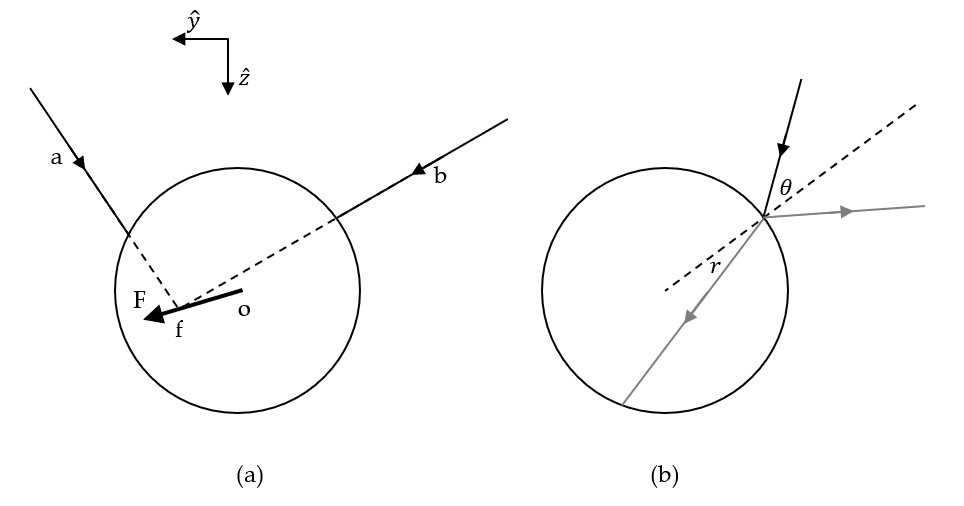
\includegraphics[width=0.8\linewidth]{../results/Optical_tweezer_illust.png}
    \caption{(a) Trap focus $f$ and the forces of dielectric sphere. (b) definition of an angle $\theta$ and $r$ in a single beam scattering}
    \label{Figure:Optical tweezer}
\end{figure}

\begin{equation}
    F_z = \frac{nP}{c} ( 1+ R \cos(2 \theta) - \frac{T^2 [\cos(2 \theta - 2r) + R \cos(2\theta)]}{1+R^2 + 2R \cos 2r} )
    \label{equation:F_z}
\end{equation}

\begin{equation}
    F_y = \frac{nP}{c} (R \sin(2 \theta) - \frac{T^2 [\sin(2 \theta - 2r) + R \sin(2\theta)]}{1+R^2 + 2R \cos 2r} )
    \label{equation:F_y}
\end{equation}
Fig. \ref{Figure:Optical tweezer}(a) illustrates that the direction of trapping force always lies to the trap focus.
We set our z direction parallel to the beam direction, and y direction as trapping focus lies on yz plane.
Equation \ref{equation:F_z} and \ref{equation:F_y} is the force by a single beam, calculated infinite sum of transmitted and reflacted light.(\cite{single_beam})
$n$ is relative refractive index, $P$ is power of the laser, $R$ is reflactance, $T$ is transmittance, $\theta$ is incident angle and $r$ is transmitted angle as Fig. \ref{Figure:Optical tweezer}(b).
I uses Fresnel equation to obtain the reflactance and transmittance of a dielectric object, and follows geometric calculation from \cite{single_beam} to numerically calculate trapping force along y axis.

\begin{figure}[t]
    \centering
    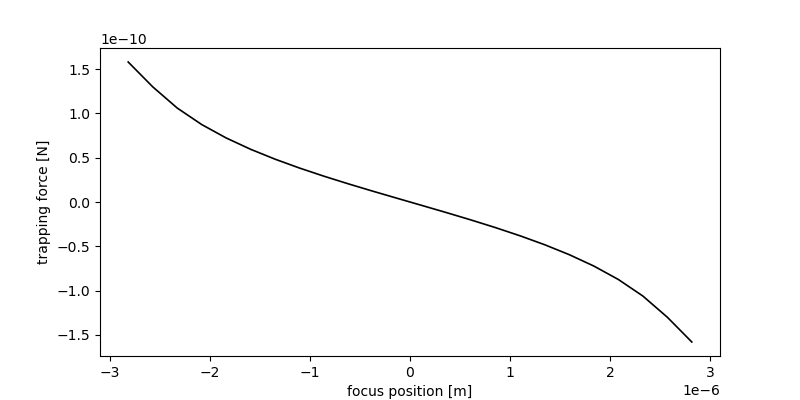
\includegraphics[width=0.8\linewidth]{../results/Optical_tweezer_intro_fig.png}
    \caption{Trapping force - focus position plot in dielectric radius $a = 3\mu m$}
    \label{Figure:Optical tweezer force}
\end{figure}

Fig. \ref{Figure:Optical tweezer force} shows the relation between trapping force and focus position. The force peaks at $0.98a$, very linear under range of $[a,-a]$.
Therefore, it is very valid to assume a trapping force as linear restoring force. I will denote trapping force $F_t = -kx$. The simulation I programmed have two module, get a force by a single beam (\verb|get_force_single_beam|), and get a total gradient force by integrating a beam given in Gaussian intensity (\verb|get_trapping_force|).
I write more details in \ref{discussion:optical_tweezer_simulation}, which whole code is uploaded in \url{https://github.com/WoojinHan24/Optical_Tweezer}

\begin{equation}
    m \ddot{x} =-b\dot{x} -k(x-vt)
    \label{equation:EOM_of_optical_tweezer}
\end{equation}
\begin{equation}
    |x(t) - vt| < a ,    \frac{vb}{k} < a 
    \label{equation:trapping criteria}
\end{equation}

Therefore, we can modelize a particle of mass $m$ and its position $x$ follows an Equation \ref{equation:EOM_of_optical_tweezer}. $v$ stands for velocity of microscope stage, which we measured in the experiments.
Equation \ref{equation:trapping criteria} shows the clear relation between trapping coefficient($k$), we want to measure, and critical velocity($v$), we had measure.


\section{Methods}
Optical tweezers module has set up in intermediate physics experiment laboratory, Seoul National University.
Total modules are made by Thorlabs, Modular Optical Tweezers kit.(\cite{opticaltweezermodule})
The experiment uses laser from Thorlabs, Inc., L658P040 - 658 nm, 40 mW (\cite{Laser_spec}).
The micro dielectric particle is made of polystyrene by Polysciences, Polybead sampler kit i, (\cite{polybead_spec}).

\subsection{Making Sample}
\noindent
Apparatus:
distilled water, polystyrene bead($1, 2, 3 [\mu m]$), micropipette, slide glass with built-in channel, cover glass

\begin{enumerate}
    \item Dillute one drop of poilystyrene bead emulsion 100 times.
    \item Drop $50 \mu l$ of the mixture in slide glass channel, carefully put a cover glass.
\end{enumerate}
The second step is very important, since the air pocket might give beads a drift force. (sample have drift force if the particle moves show tendency.)
Also the sample evaporates easily to make air layer, I have changed sample for every 30 minuates.
It is very good tip that enough mixture drop prevent those issues.

\subsection{Adjust the Focus}
\begin{figure}[h]
    \centering
    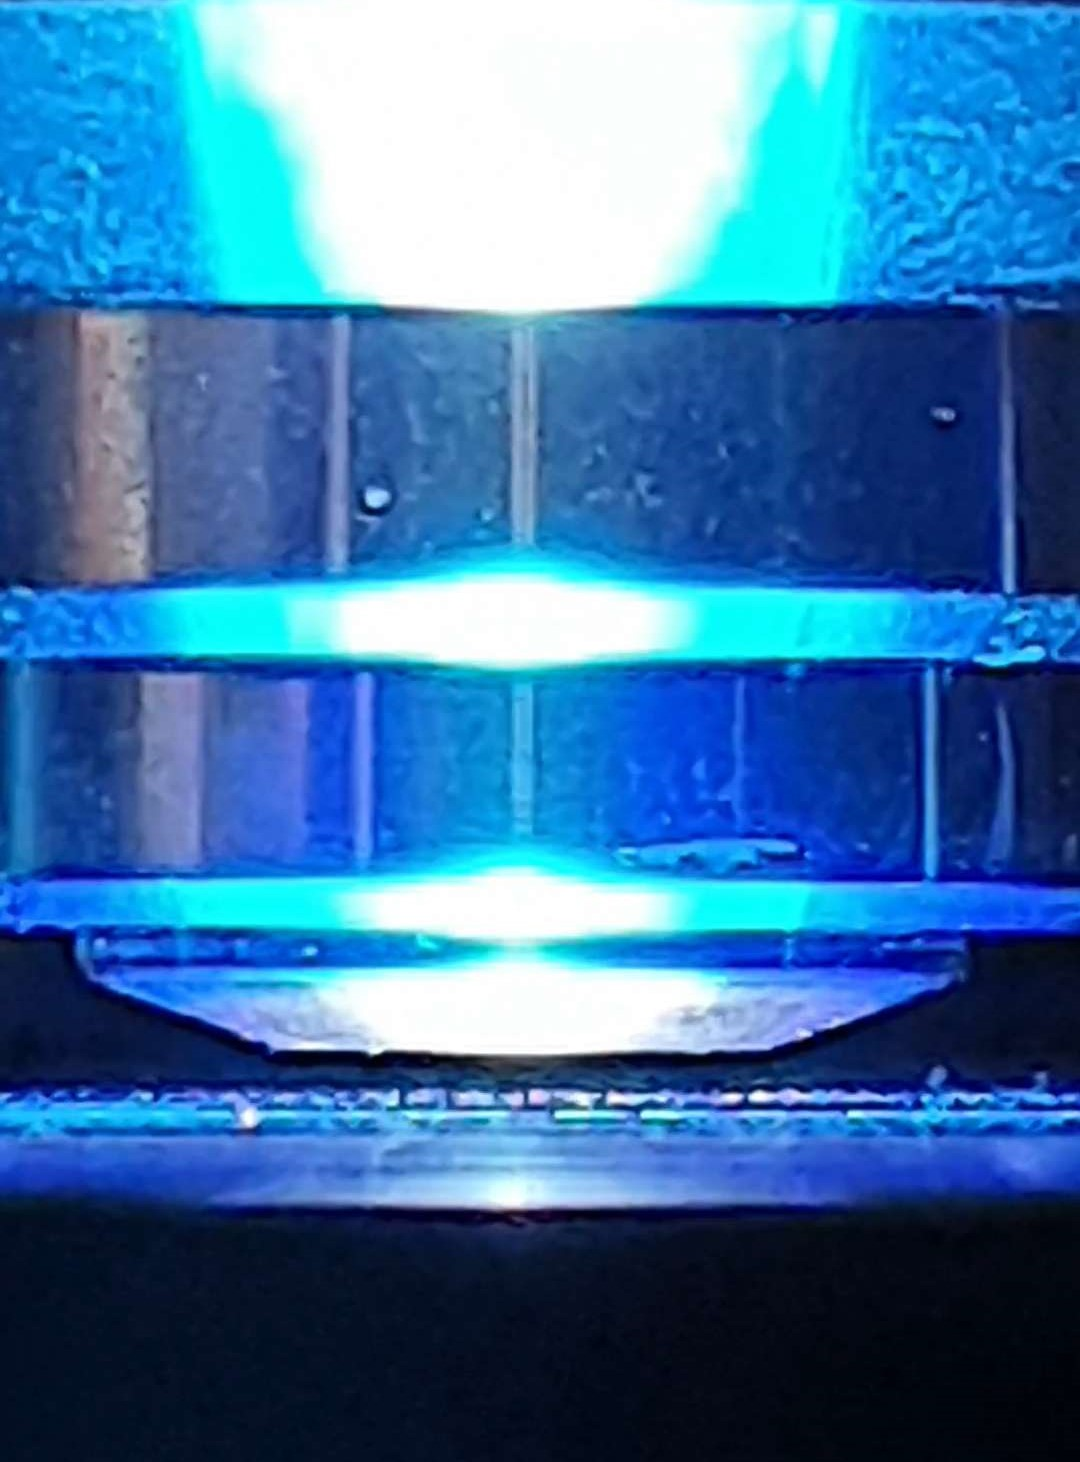
\includegraphics[width=0.3\linewidth]{../results/microscope_focusing.png}
    \caption{figure of sample and high numerical aperture objectives.}
    \label{Figure:microscope_focusing}
\end{figure}
We need a laser when adjusting the microscope focus.
The Fig. \ref{Figure:microscope_focusing} is not even close to appropriate focus, conveys that it is impossible to adjust a focus while checking the sample position.
The laser should be aligned well to make straight forward image on the sample.
In order to raise stage, three different image of laser apears.
The third and second image is so close to accidently ruins lens.
Every step below will proceed on the third focus of the laser.


\subsection{Brownian motion}
\noindent
Apparatus:
microparticle sample, Modular Optical Tweezers kit(\cite{opticaltweezermodule}), Thorcam program

\begin{enumerate}
    \item Prepare a sample, and adjust the focus.
    \item Turn on the laser and check whether a drift exsists.
    \item Mark the loction in screen and move $20-30 \mu m$ the sample to metric scale a screen.
    \item Record about 300 second of particles freely moving in fluid.
\end{enumerate}

I use tracker program to gain $(x(t),y(t))$ data of each Brownian motion.

\subsection{Measure the trapping force}
\noindent
Apparatus:
microparticle sample, Modular Optical Tweezers kit(\cite{opticaltweezermodule}), Thorcam program, sample positioning stage controller

\begin{enumerate}
    \item Prepare a sample, and adjust the focus.
    \item Move the sample stage to capture a particle.
    \item Find a critical velocity of particle, changing a stage velocity.
    \item Do 1-3 repeatly in different intensity of laser.
\end{enumerate}
I change a magnitude of current passing through the laser $30-80 mA$, which is threshold and operation current each.

\section{Results and Discussion}
\subsection{Brownian moiton : viscosity}
\label{results:brownian_motion_raw_fig}
\begin{figure}[h]
    \centering
    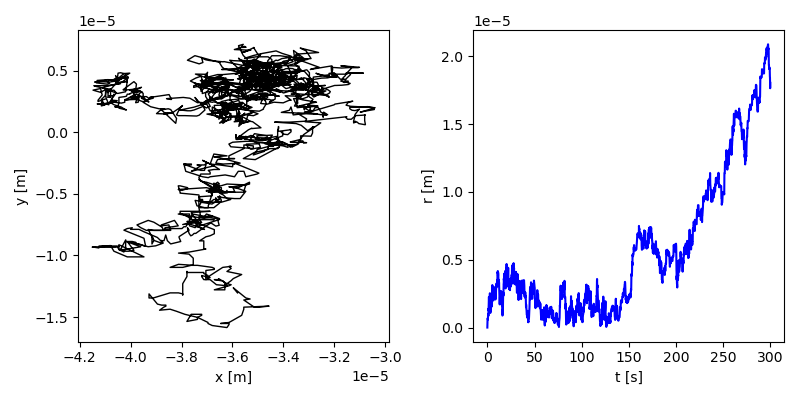
\includegraphics[width=0.8\linewidth]{../results/2um_brownian_motion_raw_fig_0.png}
    \caption{(a) raw figure of $x(t),y(t)$, (b) raw figure of $r(t)$ in experiment of $2 \mu m$ polystyrene beads}
    \label{Figure:brownian_motion_raw_fig}
\end{figure}
 Fig. \ref{Figure:brownian_motion_raw_fig} is the raw plot of the bead position.
 As the Fig . \ref{Figure:brownian_motion_raw_fig}(a) looks, it doesn't have any drift tendency.
 But for sure, I suggest \verb|Is_Drift| function whether assume sign of $\Delta x(t) = x(t) - x(0)$ follows binary distribution $B(N,1/2)$.
 If the experiment have below $20 \%$ possibility to appear, then the function returns 'True'.
 The only data in $1\mu m$ has drift tendency through those test, I neglect that data before plotting line regression.

 \begin{figure}[ht]
    \centering
    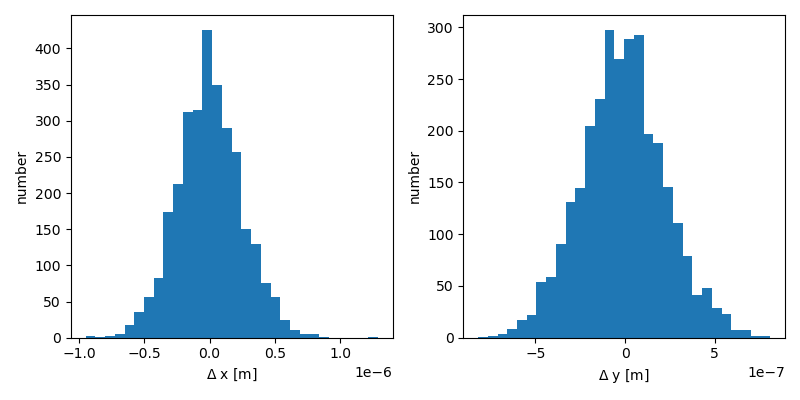
\includegraphics[width=0.8\linewidth]{../results/3um_brownian_distribution_fig_0.png}
    \caption{(a) Histogram of $\Delta x(t)$, (b) Histogram of $\Delta y(t)$ in experiment of $3 \mu m$ polystyrene beads}
    \label{Figure:brownian_motion_distribution_fig}
\end{figure}
\begin{figure}[ht]
    \centering
    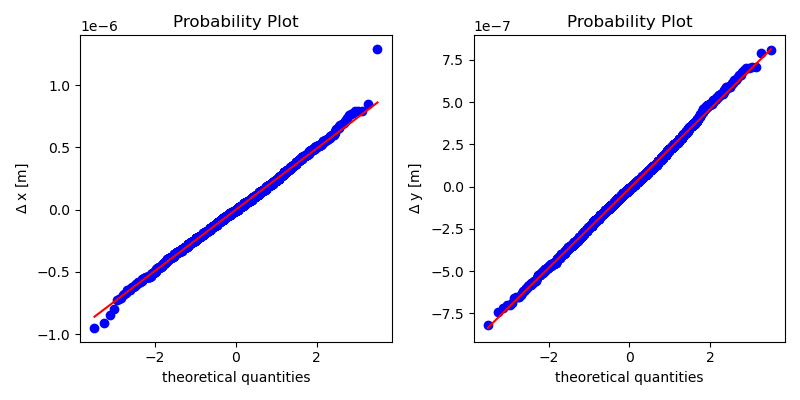
\includegraphics[width=0.8\linewidth]{../results/3um_brownian_qqplot_fig_0.png}
    \caption{(a) QQ-plot of $\Delta x(t)$, (b) QQ-plot of $\Delta y(t)$ in experiment of $3 \mu m$ polystyrene beads}
    \label{Figure:brownian_qqplot}
\end{figure}

 Moreover, the Fig. \ref{Figure:brownian_motion_distribution_fig} is the histogram result of $\Delta x(t), \Delta y(t)$ in $3\mu m$ brownian experiment.
 Fig. \ref{Figure:brownian_qqplot} is QQ-plot with normal distribution which gives hard evidence of no drift tendency.
 As a result obtain viscosity, we need to plot ensemble average to time graph.
 Polystyrene beads have $10\%$ distribution on their radius (\cite{polybead_spec}).
 For example, $2\mu m$ beads are actually contain $2 \pm 0.2 \mu m$ beads.
 It is dangerous to assume that the beads are isotropic, and merge the data in same radius to form an ensemble.
 And the method intorduced in \ref{intro:Brownian_motion} is used.
 So, I made an ensemble of each particle, gain statistical results each, and find viscosity.
 \begin{figure}[ht]
    \centering
    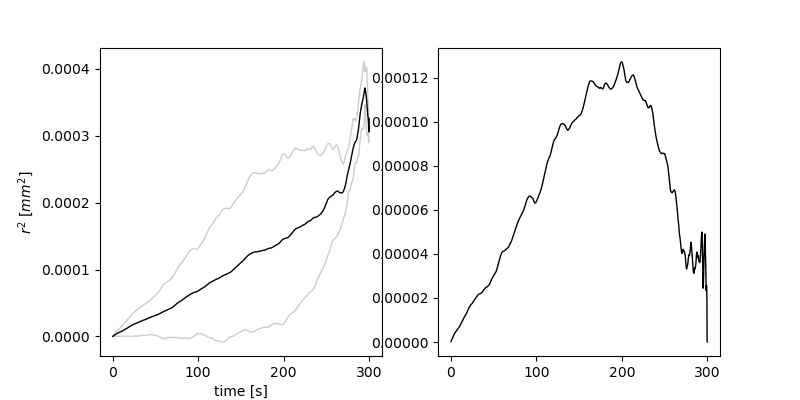
\includegraphics[width=0.8\linewidth]{../results/2um_modified_brownian_fig_0.png}
    \caption{(a) ensemble average to time plot $\bar{r^2} [m^2] - t[s]$, gray line is $1\sigma$ line, red line is linear regression result with criteria, (b) ensemble standard deviation to time plot $\sigma_{r^2} [m^2]-t[s]$}
    \label{Figure:brownian_modified_fig}
\end{figure}

The modification I've done have serious issues in end of recording time.
Ensemble $S(\tau)$ constructed by assumption of time isotropy, but their are not enough data to build ensemble for $\tau ~ t_r$.
Mathematically $(\tau-t_r)\times f$, $t_r$ is the recording time, $f$ is the frame rate, is the ensemble elements number of $S(\tau)$.
Therefore, there must be some criteria for cutting off an edge.
I suggest Einstein's theory as criteria (\cite{Brownian_motion_1}).
Einstein has suggested the ensemble variance is linear to t.
As the Fig. \ref{Figure:brownian_modified_fig}(b) has smooth linear part at front and ruined after some time comparable with the record time.
In those edge cutoff done, almost 200s (2000 frame) of data remains which is plenty enough to assume $t \gg \frac{m}{b}$, since $m$ has order of $10^{-16}$, $b$ has order of $10^{-9}$.
Plots with different size microparticle is obtained at \url{https://github.com/WoojinHan24/Optical_Tweezer/tree/master/results}.
\begin{figure}[h]
    \centering
    \begin{tabular}{|c| c| c|}
            & slopes [$m^2/s$]& viscosity [$Pa \cdot s$]\\
        \hline
        1 $\mu m$ beads & $4.70\pm 0.02 \times 10^{-12}$ & $1.40 \pm 0.01 \times 10^{-4}$\\
        2 $\mu m$ beads & $1.41\pm 0.01 \times 10^{-12}$ & $3.08 \pm 0.03 \times 10^{-4}$\\
        3 $\mu m$ beads & $6.30\pm0.09 \times 10^{-13}$ & $4.61 \pm 0.09 \times 10^{-4}$
        
    \end{tabular}
    \caption{linear regression results and viscosity in different size of beads.}
    \label{Figure:linear regression results}
\end{figure}

Linear regression results and viscosity are shown at Fig. \ref{Figure:linear regression results} in different size of beads.
By using equation \ref{equation:Brownian_motion}, slope $\alpha$ satisfies $\eta = \frac{2kT}{3\pi R \alpha}$, 2 is for degree of freedom we calculated.
I use $b = 1.56 \times 10^{-8} N\cdot s/m$ as linear drag coefficient the weighted average of the result.


\label{results:viscosity}
\label{results:modified_brownian_analysis}
\subsection{Trapping Force}
\label{results:tweezing_force}
\begin{figure}[H]
    \centering
    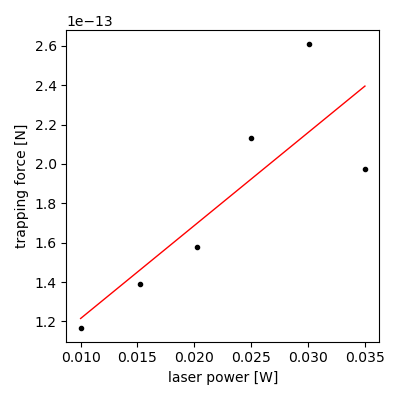
\includegraphics[width=0.32\linewidth]{../results/1um_force_raw_plot.png}
    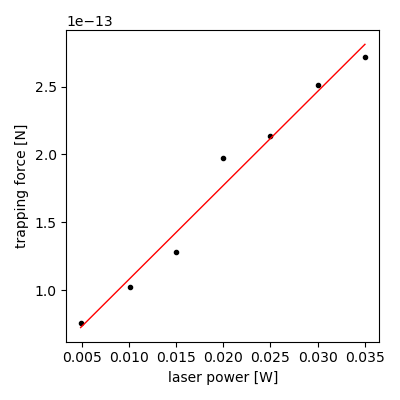
\includegraphics[width=0.32\linewidth]{../results/2um_force_raw_plot.png}
    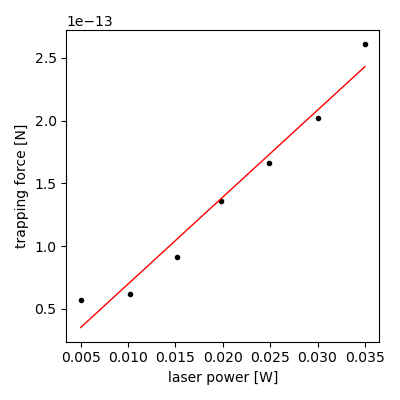
\includegraphics[width=0.32\linewidth]{../results/3um_force_raw_plot.png}
    \caption{plot of Trapping force [N] to Laser currnet [$A$](a) $1\mu m$ (b) $2\mu m$ (c) $3\mu m$, red lines are linear regression. More statics are shown below.}
    \label{Figure:force_raw_fig}
\end{figure}

In the experiment, I detect a critical velocity in function of laser current.
The laser has threshold of $35mA$ and operation current $75mA$.
At the operation current, the output power is $40 mW$ (\cite{Laser_spec})
Therefore, assuming the relation between power and current of laser follows $P= \xi  (I-I_0), I_0 = 0.035 [A], \xi = 1 [J/s\cdot A]$ is legitimate (laser has linear current dependancy to power).
\begin{figure}[H]
    \centering
    \begin{tabular}{|c| c| c|c|}
            & slopes [$1/m\cdot s$]& intercept [$N$]& $R^2$\\
        \hline
        1 $\mu m$ beads & $4.72\pm 1.3 \times 10^{-12}$ & $7.4 \times 10^{-14}$ &$R^2=0.6888$\\
        2 $\mu m$ beads & $6.92\pm 0.47 \times 10^{-12}$ & $3.87 \times 10^{-14}$&$R^2=0.9772$\\
        3 $\mu m$ beads & $6.92\pm 0.58 \times 10^{-12}$ & $5.61 \times 10^{-16}$&$R^2=0.9658$
        
    \end{tabular}
    \caption{linear regression results of Fig. \ref{Figure:force_raw_fig} in different size of beads.}
    \label{Figure:force power linear regression results}
\end{figure}

The experiment on 1 $\mu m$ beads is too hard to measure since the particle are rarly catchable.
But the two different results are highly accurate, so I will compare those results with simulations.

\subsection{optical tweezer model}
\label{discussion:optical_tweezer_simulation}
\begin{figure}[h]
    \centering
    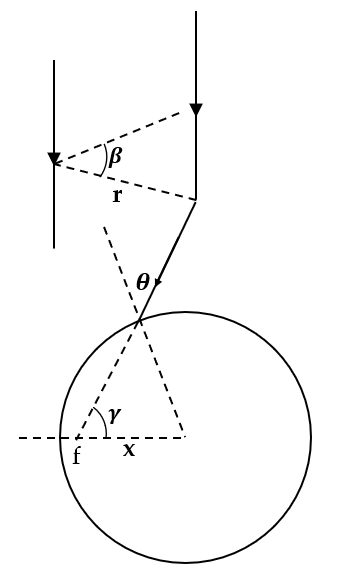
\includegraphics[width=0.3\linewidth]{../results/Optical_tweezer_simulation_fig.png}
    \caption{Geometric relation of optical tweezer simulation}
    \label{Figure:optical tweezer simulation_fig}
\end{figure}
Fig \ref{Figure:optical tweezer simulation_fig} shows geometrical reference of my calculation.
First, The laser comes downward from lens makes its focus on point $f$.
And, the intensity is relavent to its relative position with the center of the laser.
In figure, $r$ is the relative distance from laser axis, and angle $\beta$ denotes direction form some axis.
Therefore the single beam in the laser incident with angle $\theta$, gives force to dielctric in terms of equation \ref{equation:F_z} and \ref{equation:F_y}.
I numerically integrate the total force by $r$ and $\beta$ in direction of $x$ and plot in Fig. \ref{Figure:Optical tweezer force}.
(\cite{single_beam}, \url{https://github.com/WoojinHan24/Optical_Tweezer/blob/master/optical_tweezer.py})
The laser and module specs were all open in \cite{opticaltweezermodule}, focus depth $f= 1 \mu m$, Numerical apperature $N/A =1.25$.



\subsection{Refractive index}
\label{discussion:refractive_index_calculation}
I suggest the mathematical method to calculate refractive index with optical tweezer.
This method is imperfect since lack of the dataset, but it is still notable to others try afterall.
In above experiments, for critical velocity $v$ and $P$, $\frac{d v}{dP}$ has calculated.
Using criteria at equation \ref{equation:trapping criteria}, 
\begin{equation}
    \frac{dk}{dP} = \frac{1}{R} \frac{d (bv)}{dP}
\end{equation}
The linear trapping force coefficient $k$ has been measured and also simulated.
For the laser radius is $5.6 mm$, the magnification $\times 100$ is considered to find gaussian distribution precisely.
At  fig. \ref{Figure:final_fig}, the simulation results of $\frac{dk}{dP}$ is plotted on differ by refraction index.
\begin{figure}[h]
    \centering
    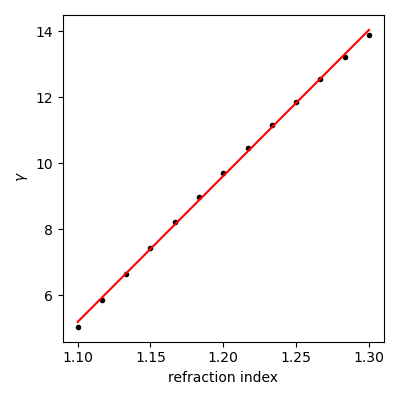
\includegraphics[width=0.3\linewidth]{../Final_figure.png}
    \caption{$\frac{dk}{dP} [10^{-6} /m^2 \cdot s]$ to n plot}
    \label{Figure:final_fig}
\end{figure}

After the linear regression, $\frac{dk}{dP} = (44.3 n  -43.5)\times 10^{-6} = (3.45 \times 10^{-6}) [1/m^2 \cdot s]$ for 2 $\mu m$ beads.
Therefore, in that experiment, I obtained the relative refractive index as 1.05, which real value lies on $1.58/1.33 = 1.18$.
But it is very difficult to numerically find standard deviation of that results, it is impossible to declare any statistical verification in this results.
Any changes of this calculation or simulation will be updated in Github.

\section{Summary}
The brownian motion and its ensemble modification has applied. Therefore, the viscosity value and the linear drag coefficient has obtained.
The trapping criteria and optical tweezer simulation has proceeded, the plot has successfully explain the trapping phenomena.
Furthermore, the refractive index calculation is suggested and applied.
It was not very successful to make accurate assumption of the index, it has a lot of oppertunity to develop.

\bibliography{optical_tweezer_ref}
\bibliographystyle{plain}
\end{document}